%%%% ijcai17.tex

\typeout{IJCAI-17 Instructions for Authors}

% These are the instructions for authors for IJCAI-17.
% They are the same as the ones for IJCAI-11 with superficical wording
%   changes only.

\documentclass{article}
% The file ijcai17.sty is the style file for IJCAI-17 (same as ijcai07.sty).
\usepackage{ijcai17}
% Use the postscript times font!
\usepackage{times}
\usepackage{multirow}
\usepackage{multicol}
\usepackage{array}
\usepackage{graphicx}
\usepackage[outdir=./]{epstopdf}
\usepackage{footnote}
\makesavenoteenv{table}
\usepackage{amsmath, bm}
\usepackage{url}


% the following package is optional:
%\usepackage{latexsym} 

% Following comment is from ijcai97-submit.tex:
% The preparation of these files was supported by Schlumberger Palo Alto
% Research, AT\&T Bell Laboratories, and Morgan Kaufmann Publishers.
% Shirley Jowell, of Morgan Kaufmann Publishers, and Peter F.
% Patel-Schneider, of AT\&T Bell Laboratories collaborated on their
% preparation.

% These instructions can be modified and used in other conferences as long
% as credit to the authors and supporting agencies is retained, this notice
% is not changed, and further modification or reuse is not restricted.
% Neither Shirley Jowell nor Peter F. Patel-Schneider can be listed as
% contacts for providing assistance without their prior permission.

% To use for other conferences, change references to files and the
% conference appropriate and use other authors, contacts, publishers, and
% organizations.
% Also change the deadline and address for returning papers and the length and
% page charge instructions.
% Put where the files are available in the appropriate places.

\title{Learning to Extract Events without Human-annotated Text}

\begin{document}

\maketitle

\begin{abstract}
Existing event extraction systems are typically based supervised learning over expert-annotated datasets.
%Due to the drastic efforts involved in annotation, these datasets often only provide  limited event types.
%such as ACE and ERE event extraction frameworks.
However, designing and constructing these
high-quality corpora, even with limited size and coverage of event types,  is costly.
This makes learned extractors hard to generalize.  With the essence of distant supervision,
%Inspired by some Freebase schemas which share similar structures with ACE event templates,
we investigate the possibilities of automatic construction of training data for various event types
with the help of structured knowledge bases.
%the following problems in this paper: can we generate a feasible dataset for event extraction with Freebase automatically and is it possible to extract events on this dataset.
%We first propose four hypotheses based on our observation and produce our dataset accordingly. Then,
We further propose a novel neural network with ILP-based post inference committing to
handling two challenges in event extraction: multi-type events and multi-word arguments.
Both automatic and manual evaluations demonstrate that it is possible to learn to extract various  events, according to existing knowledge bases, without human-annotated training data.
\end{abstract} 

\section{Introduction}
%Automatically extracting events from natural text is an outstanding challenging task in information extraction.
Event extraction from text is an important, underpinning technique for many natural language processing tasks.
Among diverse types of event extraction systems, the extraction task proposed by Automatic Content Extraction (ACE)
\cite{doddington2004automatic} is the most popular framework, which defines two main terminologies: \textbf{trigger}
and \textbf{argument}. The former is the word that most clearly expresses the occurrence of an event. The latter is a
phrase that serves as a participant or attribute with a specific role in an event.

Constructing training data for the ACE task currently requires heavy human involvement. To do so, linguists will first
summarize a large amount of text to generate a set of design templates about potential arguments for each event type;
then human annotators will be employed to manually label the text using the templates. The problem here is that human
annotators often generate inconsistent triggers or arguments. Consider the the question, can a prepositional phrase or
a portion of a word trigger an event, e.g., \textit{in prison} triggers an \emph{arrest} event, or, \textit{ex} in
\textit{ex-husband} triggers a \emph{divorce} event? Different annotators could give different answers event for the
same sentence. What we would like to have is an automatic way to generate consistent training data, because manual labeling is
expensive and
the contradictory data can severely affect the performance of the ACE task.

In addition to the challenge of training data generation, current ACE event extraction systems
also have two major drawbacks -- they can only support single-token trigger labeling and have
a one to one mapping from a type to an event. These restrictions make these ACE event extraction
systems in applicable when. \todo{give an example.}

%Constructing high-quality training data for the ACE task is expensive, requiring heavy human involvement. This
%typically consists of two steps. First, linguists are required to summarize a large amount of text to elaborately design
%templates about potential arguments for each event type. Second, rules should be explicitly stated to guide annotators.
%Even with detailed guidelines, there is often disagreement among human annotators about what should (not) be regarded
%as triggers/arguments. For example, can a prepositional phrase or a portion of a word trigger an event, e.g.,
%\textit{in prison} triggers an \emph{arrest} event, or, \textit{ex} in \textit{ex-husband} triggers a \emph{divorce}
%event? Furthermore, current ACE event extraction systems have two major limitations, i.e., they can only have
%single-token trigger labeling and a one to one mapping from a type to an event.
%These limitations restrict the wide adoption of ACE event extraction systems at scale.


%The aforementioned drawbacks of ACE event extraction systems motivate us to
This paper addresses the two problems mentioned above. More specifically, we try answer the following two questions:
(1) can we automatically build a dataset for event extraction without experts involved?
and (2) can we have an event extractor that handles more realistic scenarios, e.g.,  when trigger annotations are unavailable, or events with more than one type.


%It would be interesting to see (1) can we automatically build a dataset for event extraction without experts involved?
%and (2) can we have an event extractor that handles more realistic scenarios, e.g.,  when trigger annotations are unavailable, or events with more than one type.

To tackle the problem of training data generation, we use distant supervision learning to extract knowledge from structured knowledge bases (KBs) 
to automatically generate training examples. 
Recent studies \cite{mintz2009distant,zeng2015distant} ave demonstrated the
effectiveness of applying distant supervision to KBs for binary relation extraction. While promising, 
there are two major hurdles for leveraging KB to event extraction. Firstly, event structures are more complex than 
binary relations. They can be
represented as $\langle event\_type, argument_1, \ldots, argument_n\rangle$, which are n-ary relations with various
numbers of arguments. Secondly, there is no explicit trigger information in any existing knowledge base for distant 
supervision to learn over. Our key insight to the problems is that for a particular event type, there is a group of
\textbf{key arguments} which together can imply an event instead of explicit triggers. \todo{what about the structure problem?}
In this work, we utilize Freebase as our
knowledge base and Wikipedia articles as text for data generation. We show that our solutions can yield \todo{high quality training data for event extraction?} . 


%This is based on our observation that KBs often organize complex structured information in tables, which
%share similar structures with ACE event definitions. An entry of such tables usually implies the occurrence
%of certain events. On the other hand, recent studies \cite{mintz2009distant,zeng2015distant} have demonstrated the
%effectiveness of KB as distant supervision for binary relation extraction. However, there are two major challenges when
%leveraging KB to event extraction: first, event structures are more complex than binary relations. They can be
%represented as $\langle event\_type, argument_1, \ldots, argument_n\rangle$, which are n-ary relations with various
%numbers of arguments. Second, there is no explicit trigger information in any existing knowledge base. Therefore, to
%explore the distant supervision (\texttt{DS}) assumption in event extraction, we investigate different hypotheses for
%better data quality and quantity. Among them, the vital one is that, for a particular event type, there is a group of
%\textbf{key arguments} which together can imply an event instead of explicit triggers. We utilize Freebase as our
%knowledge base and Wikipedia articles as text for data generation. According to Mintz et al.
%\shortcite{mintz2009distant}, because a major source of Freebase is the tabular data from Wikipedia, making it a
%natural fit with Freebase. Figure~\ref{fig:3} illustrates examples of sentences annotated by our algorithm.

To overcome the restrictions of the current ACE systems, we propose a novel event extraction paradigm with key
arguments to characterize an event type. We consider event extraction as two sequence labeling subtasks, namely event
detection and argument detection. Inspired by neural network models in sequence labeling tasks
\cite{huang2015bidirectional,lample2016neural}, we utilize LSTM-CRF models to label key arguments and non-key arguments
in the each sentence separately. However, event structures are not simple sequences and there are strong dependencies
among key arguments. We therefore reformulate the hypotheses as constraints, and apply linear integer programming to
output multiple optimal label sequences to capture multi-type events. We show that our solution leads to better performance,
representing a significant departure from the prior works for the ACE task seen to date~\cite{ahn2006stages,li2013joint,chen2015event,nguyen2016joint}.

%Second, unlike previous studies that focus on tasks defined by ACE evaluation framework
%\cite{ahn2006stages,li2013joint,chen2015event,nguyen2016joint}, we propose a novel event extraction paradigm with key
%arguments to characterize an event type. We consider event extraction as two sequence labeling subtasks, namely event
%detection and argument detection. Inspired by neural network models in sequence labeling tasks
%\cite{huang2015bidirectional,lample2016neural}, we utilize LSTM-CRF models to label key arguments and non-key arguments
%in the each sentence separately. However, event structures are not simple sequences and there are strong dependencies
%among key arguments. We therefore reformulate the hypotheses as constraints, and apply linear integer programming to
%output multiple optimal label sequences to capture multi-type events.

%In this paper, we exploit existing structured knowledge bases, e.g., Freebase, as distant supervision to automatically
%annotate event structures from plain text without human annotations. We further propose a novel event extraction
%paradigm that harnesses key arguments to imply certain event types without explicit trigger annotations. We present an
%LSTM-CRF model with post inference to extract both Freebase-style events as well as multi-type event mentions on the
%generated dataset, which is demonstrated effective by both manual and automatic evaluations.

We apply our approach to \todo[xx}. Evaluation results show that \todo{xx}. The key contributions of this work are 
(1) a  novel event extraction paradigm that harnesses key arguments to imply certain event types without explicit trigger annotations,
and (2)  an LSTM-CRF model with post inference to extract both Freebase-style events as well as multi-type event mentions on the
generated dataset. Our approach is shown to be effective in both manual and automatic evaluation tasks. 


\section{Dataset Preparation}
Here, we will employ the event-related entries in Freebase~\cite{bollacker2008freebase}  to automatically annotate \red{event descriptions} in Wikipedia's pages, with the essence of  \texttt{DS}. We regard a sentence as positive when it mentions the occurrence of an event, or otherwise negative. For example, S1 and S2 are positive examples with their arguments in italics and underlined (also shown in Figure~\ref{fig:3}), while S3 and S4 are negative. 
%The event structures of S1 and S2 are illustrated in Figure~\ref{fig:3}.
%
\begin{quote}
	\textbf{S1}: \underline{\emph{Remedy Corp}} was sold to \underline{\emph{BMC Software}} as the \underline{\emph{Service Management Business Unit}} in \underline{\emph{2004}}.
\end{quote}
\begin{quote}
	\textbf{S2}: \underline{\emph{Microsoft}} spent \$6.3 billion buying online display advertising company \underline{\emph{aQuantive}} in \underline{\emph{2007}}.
\end{quote}
\begin{quote}
	\textbf{S3}: Microsoft hopes aQuantive's Brian McAndrews can outfox Google.
\end{quote}
\begin{quote}
	\textbf{S4}: On April 29th, Elizabeth II and Prince Philip witnessed the marriage of Prince William.
\end{quote}
%
\subsection{Freebase}
Freebase is a structured knowledge base, which can be divided into three layers: \emph{domain}, \emph{type} and \emph{instance}. \emph{Instances} are entries in Freebase, and related to real-world entities\red{ and their relationship??}. \emph{Types} are different perspectives of \emph{instances}. \textbf{\emph{Compound Value Type}} (CVT) is a special type in Freebase to represent complex structured data where instances \red{ are described with} multiple \textbf{\emph{properties}}, usually organized in a table. Some of the CVT schemas indeed imply certain events, e.g., \red{\emph{divoice??sports related???} and \emph{business.acquisition}} , and  closely resemble to event structures, where CVT properties can be treated as event arguments. As shown  in Figure~\ref{fig:3},
% \emph{business.acquisition} is a CVT whose properties are \emph{company\_acquired}, \emph{acquiring\_company}, \emph{date} and \emph{divisions\_formed}. 
the properties of CVT  \emph{business.acquisition}  actually can be used to \red{lable/indicate}  %can be used to represent 
the participants and attributes of the events mentioned in S1 and S2.

We use the Freebase copy of 2013-06,  %version of Berant et al. \shortcite{berant2013semantic}, 
containing 1010 CVTs. After filtering out those %CVTs that 
describing the Freebase structures  or irrelevant to events (e.g., \emph{food.recipe\_ingredient}), we obtain 24 CVTs with around 280 million instances.    
%
\begin{figure}[h]
	\centering
	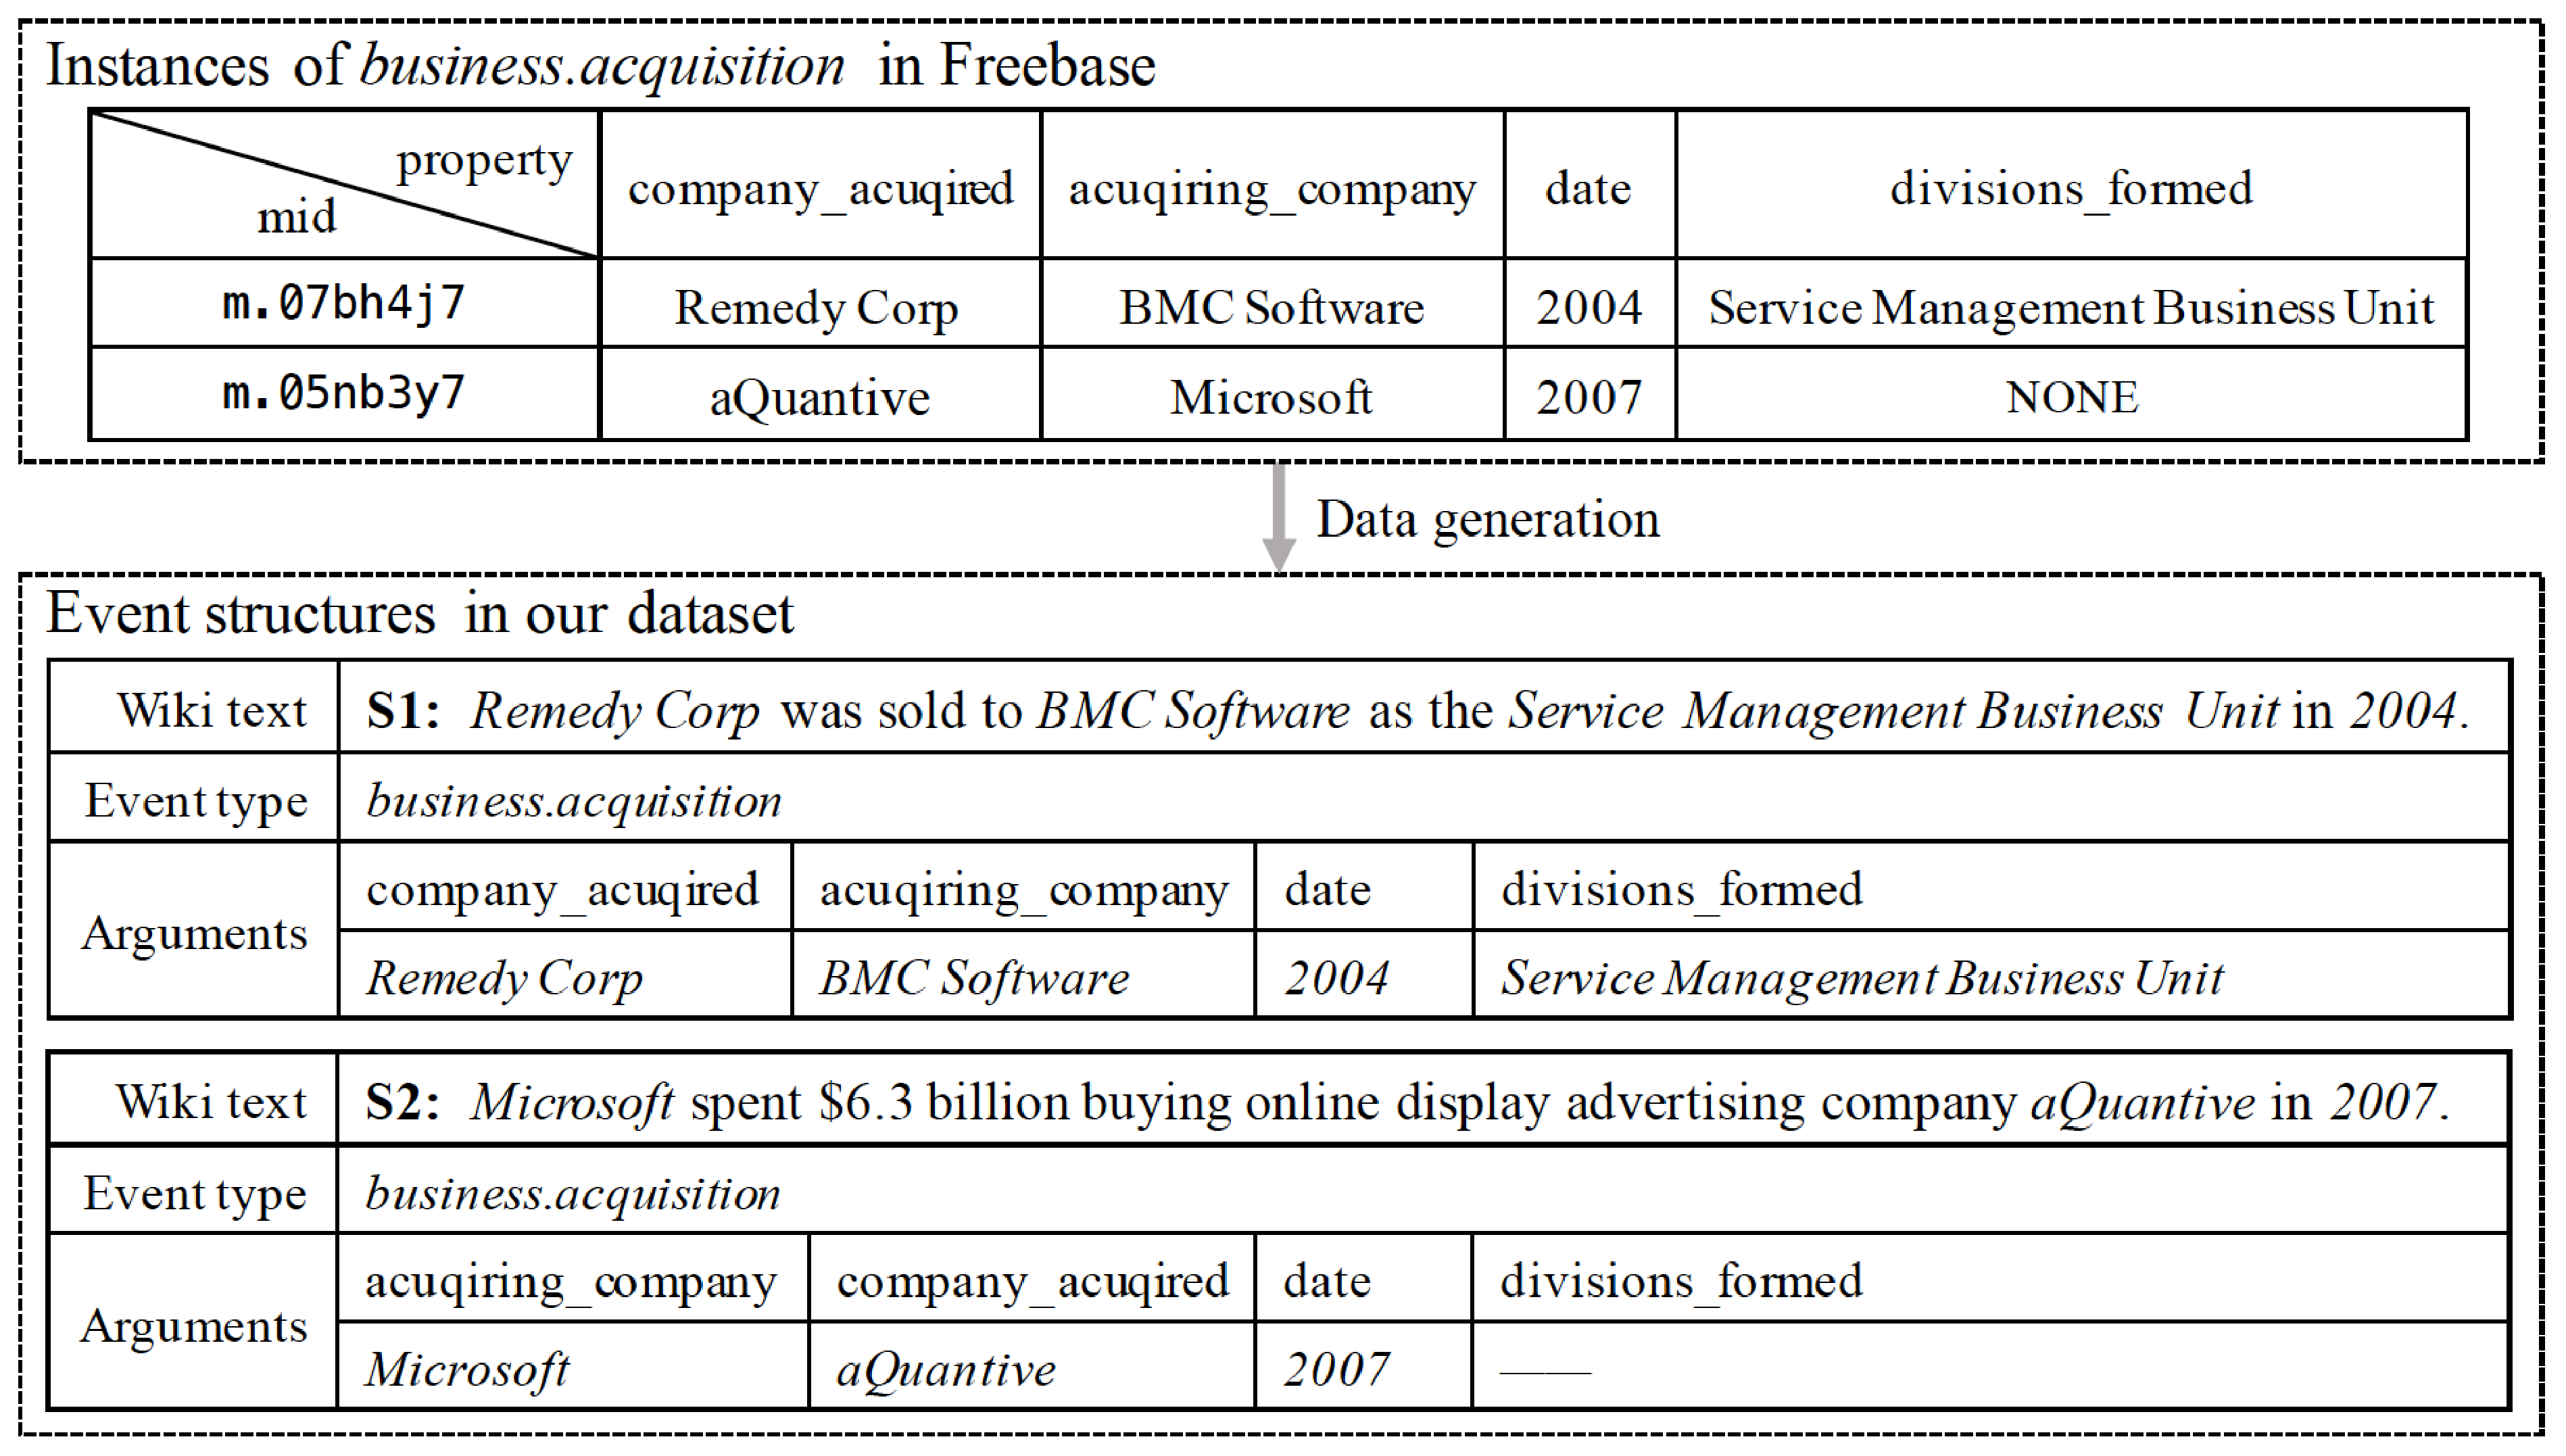
\includegraphics[width=.48\textwidth]{temp}
	\caption{Examples of CVT instances in Freebase, and labeled sentences in our dataset. \emph{Company\_acuqired}, \emph{acquiring\_company} and \emph{date} are key arguments in \emph{business.acquisition}. \label{fig:3}}
\end{figure}

\subsection{Data Generation\label{datagen}}
Now we will describe how to automatically collect training data with quality event annotations, by pushing forward the \texttt{DS} framework.
\subsubsection{H1: Positive sentences should contain all properties}
Our first hypothesis is that \textit{if a sentence contains all properties of an entry in a CVT, this sentence will be 
considered as a positive instance to indicate an event of such type characterized by this CVT}.  
We will then label the sentence as a mention of this CVT event, and the words or phrases that 
match this entry's properties as the involved arguments, with the roles specified by their 
corresponding property names. 
For example, S1 contains all the properties of instance $m.07bh4j7$ with a CVT type \emph{business.acquisition}, 
we thus consider S1 as a positive instance implying an event about \emph{business.acquisition}, and \emph{BMC Software}, \emph{Remedy Corp}, \emph{Service Management Business Unit} and \emph{2004} will be labeled as the arguments that play the role of \emph{acquiring\_company}, \emph{company\_acquired}, \emph{divisions\_formed}, and \emph{date} in this event, respectively.

%However, in practice, we realize that \emph{H1} is too strict that excludes a great many positive sentences like S2. 

\subsubsection{H2: Positive sentences should contain all key properties}
In practice, we find that \emph{H1} is too strict to include many positive instances like S2. 
We thus relax \emph{H1} by replacing \textbf{all properties} with \textbf{\red{all??????} key properties}. We define the CVT property that plays an important part in its CVT structure and helps to distinguish with other CVTs as a \textbf{key property}. A \textbf{key argument} is the word/phrase that matches a key property of a CVT instance. For example, \emph{company\_acquired} and \emph{acquiring\_company} are the key properties of CVT \emph{business.acquisition}, therefore,  S2 should be a positive instance for a \emph{business.acquisition} event, since it contains all key properties. Table~\ref{tab:5} lists the key properties of four CVTs.

The importance of a property $prop$ (e.g., \emph{date}) to its CVT $cvt$ (e.g., \emph{business.acquisition}) can be defined as:
\begin{equation}
	degree_{cvt, prop} = log \frac{count(cvt, prop)}{count(cvt) \times count(prop)} 
\end{equation}
where $count(cvt)$ is the number of all instances of type $cvt$, $count(prop)$ is the number of times $prop$ appearing in all CVTs, and $count(cvt, prop)$ is the number of $cvt$ instances that contain the property $prop$.

\begin{table}
\centering
\small
\begin{tabular}{|l|l|} \hline
CVT & Key properties \\ \hline
award.award\_honor & award\_winner, award, \ldots, year \\ \hline
film.performance & actor, film, character \\ \hline
education.education & institution, student, end\_date \\ \hline
business.employment\_tenure & company, title, person, from \\ \hline
\end{tabular}
\caption{Examples of key properties of four CVTs.\label{tab:5}}
\end{table}

\subsubsection{H3: Key properties should include time-related property}
%We discover that for many CVTs, their key properties do not take into account time property. 
Although time-related arguments are often missing in the currently imperfect KBs, time-related properties are indeed
crucial to indicate an actual event mention, e.g., S3, containing  \emph{Microsoft} as \emph{acquiring\_company} and \emph{aQuantive} as \emph{company\_acquired} but without time-related arguments, should not be considered as a negative example for
event \emph{business.accquisition}.
% while contain all key properties of an instance, resulting in mistaking \emph{Microsoft} for \emph{acquiring\_company}, and \emph{aQuantive} for \emph{company\_acquired}. 
%By adding \emph{date} to the set of key properties, S3 will be filtered. 
We thus include the time-related properties with the highest importance scores  as supplementary key properties. 

\subsubsection{H4: Positive sentences should contain key properties with close syntactic distance}
We introduce another factor, syntactic distance, to annotate positive sentences. Intuitively, two arguments participant in the same event are likely to have close syntactic distance. This factor is effective to eliminate negative sentences, such as S4. The syntactic distance can be measured by the distance of two words in dependency parsing tree. We set the maximum distance between two key arguments as 2, denoting that, for a candidate sentence, if a pair of key arguments violates this constraint, it is supposed to be negative. Given the dependency parsing tree in Figure~\ref{fig:2}, S4 is negative because the distance between \emph{Prince Philip} and \emph{marriage} is 3.

\begin{figure}
	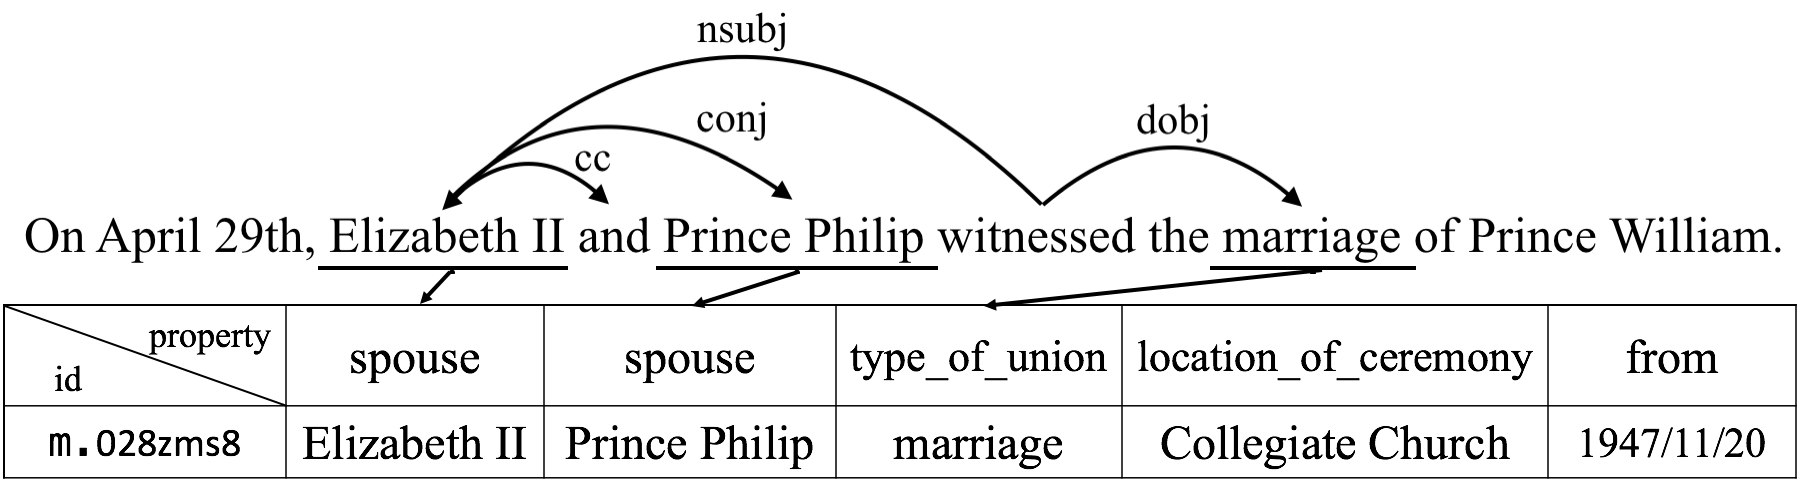
\includegraphics[width=.48\textwidth]{deppath}
	\caption{An illustration of dependency parse tree of S4. \label{fig:2}}
\end{figure}

We conduct a manual evaluation on the quantity and quality of  datasets generated by different hypotheses (see Section~\ref{sec:evalhypo}), and utilize the combinations of hypothesis \emph{H3} and \emph{H4} as the final strategy.

\section{Model}
Unlike existing event extraction work in which triggers are the key evidence to identify event and classify different event types, in the absence of human-labeled triggers, we argue that \textbf{key arguments} can play the same role as triggers. Consequently, we can treat event extraction as a pipeline of two primary subtasks, namely event detection and argument detection.

\noindent \textbf{Event detection}: to identify key arguments in the sentence. And if a sentence contains \textbf{all} key arguments of a specific event type, it is considered to imply an event of the corresponding type. For example, in S1, \emph{Remedy Corp}, \emph{BMC Software}, and \emph{2004} should be identified as \emph{business.acquisition.company\_acquired}, \emph{business.acquisition.acquiring\_company}, and \emph{business.acquisition.date} respectively. As a result, S1 should be labeled as expressing an event about \emph{business.acquisition}.

\noindent \textbf{Argument detection}: to identify other non-key arguments for each event in the sentence. For the \emph{business.acquisition} event in S1, \emph{Service Management Business Unit} should be identified as \emph{business.acquisition.divisions\_formed}.

\subsection{Event Detection \label{evede}}
Before presenting our model, we need to come up with the solution to multi-words arguments. Then we introduce the components in our LSTM-CRF-ILP$_{multi}$ model one-by-one from bottom to top.

\paragraph{Tagging scheme}
68 percent of arguments in our dataset consist of more than one words. To address this issue, we model each subtask as a sequence labeling task rather than a word classification task. Each word in the given sentence is tagged in the \texttt{BIO} scheme, where each token is labeled as \texttt{B-role} if it is the beginning of an event argument with its corresponding role \texttt{role}, or \texttt{I-role} if it is inside an argument, or \texttt{O} otherwise. 

\paragraph{LSTM}
Long Short-Term Memory Network (LSTM) \cite{hochreiter1997long} is a natural model for sequence labeling task, which maintains a memory based on historical contextual information. Formally, given a sentence $\bm{w} = \{w_1, w_2, \dots, w_n\}$ of length $n$, we use $\textbf{x}_t$ to represent feature vector (e.g. word embedding) corresponding to the $t$-th word $w_t$. At each time step $t$, a LSTM unit takes $\textbf{x}_t$ as input and computes the output vector $\textbf{h}_t$ through several multiplicative gates. Then output vector is fed into a softmax layer to estimate a probability distribution over all possible labels.

\paragraph{CRF}
A straightforward way is to choose the label which obtains maximum probability by LSTM as the prediction for each word. However, this independent labeling strategy is limited especially when there are strong dependencies and constraints between arguments.
% For instance, \texttt{B-acquiring\_company} is more likely to be followed by \texttt{B-company\_acquired}, while \texttt{I-company\_acquired} is not allowed to follow \texttt{B-acquiring\_company}. 
To model the correlations between labels, we introduce a CRF layer into the output of LSTM, which is widely used and proved to be effective in various sequence labeling tasks, such as POS tagging and NER \cite{collobert2011natural,huang2015bidirectional,lample2016neural}.

We consider $\textbf{P}$ to be a matrix of confidence scores output by LSTM network, and the element $\textbf{P}_{i,j}$ of the matrix denotes the probability of the label $j$ for the $i$-th word in a sentence. The CRF layer has a transition score matrix $\textbf{A}$ as parameter, where $\textbf{A}_{i,j}$ represents the score of a transition from label $i$ to label $j$. The score of a sentence $\bm{w}$ along with a path of labels $\bm{y} = \{y_1, y_2, \ldots, y_n\}$ is measured by the sum of neural network outputs and transition scores: 
\begin{equation}
	score(\bm{w}, \bm{y}) = \sum\limits_{i=0}^n\textbf{P}_{i, y_i} + \sum\limits_{i=1}^n\textbf{A}_{y_i, y_{i+1}},
\end{equation}
During test, given a sentence $\bm{w}$, we adopt the Viterbi algorithm \cite{rabiner1989tutorial} to find the optimal label sequence with the maximum score among all possible label sequences.

\paragraph{ILP-based Post Inference}
Event detection is a structure prediction problem, while the output sequences of LSTM-CRF not necessarily satisfy the structural constraints. Specifically, regardless of how many key arguments are identified correctly by LSTM-CRF, if there is one key argument missing, detection of its corresponding event is failed. To amend this flaw, we apply Integer Linear Programming (ILP) with respect to the scores given by the above LSTM-CRF model to generate the final labeling sequence.

Formally, let $\mathcal{L}$ be the set of possible argument labels. For each word $w_i$ in the sentence $\bm{w}$ and a pair of labels $ \langle l, l' \rangle \in \mathcal{L} \times \mathcal{L}$, we create a binary variable ${v_{i,l,l'} \in \{0, 1\}}$, denoting whether or not the $i$-th word $w_i$ is tagged as label $l$ and its following word $w_{i+1}$ is tagged as label $l'$ at the same time. The objective of ILP is to maximize the overall score of the variables,
\begin{displaymath}
	\sum\nolimits_{i, l, l'}v_{i,l,l'} * (\textbf{P}_{i,l}+\textbf{A}_{l,l'}) .
\end{displaymath}

We consider the following four constraints:

\textbf{C1}: Each word should be and only be labeled with one label, i.e.:
\begin{equation}
	\sum\nolimits_{l,l'}v_{i,l,l'}=1
\end{equation}

\textbf{C2}: If the value of $v_{i,l,l'}$ is $1$, then there has to be a label $l^*$ which makes $v_{i+1,l',l^*}$ equal to $1$, i.e.:
\begin{equation}
	v_{i,l,l'} = \sum\nolimits_{l^*}v_{i+1,l',l^*}
\end{equation}

\textbf{C3}: If current label is \texttt{I-arg}, then its previous label must be \texttt{B-arg}, i.e.:
\begin{equation}
	v_{i,\texttt{I-arg},l'} = v_{i-1,\texttt{B-arg},\texttt{I-arg}}
\end{equation}

\textbf{C4}: For a specific event type, its key arguments should be co-occurred, or none of them should appear in the resulting sequence. For any pair of key arguments $arg_1$ and $arg_2$ with respect to the same event type, the variables related to them are subject to:
\begin{equation}
	\sum\nolimits_{i,l'}{v_{i,\texttt{B-arg}_1,l'}} \leq n * \sum\nolimits_{j,l^*}{v_{j,\texttt{B-arg}_2,l^*}}
\end{equation}
where $n$ is the length of the sentence.

In order to address the multi-type event issue, we design a heuristic approach that iteratively produces new label sequences based on the following constraint \textbf{C5}.

\textbf{C5}: We eliminate all resulting sequences solved by ILP in the past iterations from the solution space, to obtain the next optimal sequences, i.e., for a specific sequence produced at iteration $t$, $\bm{s}^t=\{l_1^t, l_2^t, \ldots, l_n^t\}$,  
\begin{equation}
	\forall i \in {[0, n)}, v_{i,l_i^t ,l_{i+1}^t} = 0	
\end{equation}

We repeat the above procedure with these constraints through ILP, until the difference between objective value of $\bm{s}^1$ and $\bm{s}^T$ is greater than a threshold $\lambda$. Finally, we consider all sequences $\{\bm{s}^1, \bm{s}^2, \ldots, \bm{s}^{T-1}\}$ as the optimized set of label sequences. In our experiment, Gurobi \cite{gurobi} is chosen as our ILP problem solver and $\lambda=0.05 \times n$.

\subsection{Argument Detection}
After event detection, a sentence will be classified into different event types, and labeled with its corresponding key arguments. Next step is argument detection which aims to identify the remaining arguments (non-key arguments) in the sentences.  

We simply adapt the input embeddings of the LSTM-CRF model (see Section~\ref{evede}) for argument detection. Given an input sentence and one of its label sequence produced from upstream event detection task, we encode the label of each word into a key-argument feature vector through a look-up table. Then, we concatenate the word vector and key-argument feature vector as the input vector to LSTM. And no more post inference is needed in this subtask.

\section{Experiments}

\subsection{Experimental Setup}
\paragraph{Dataset and Evaluation Methodology}
We use the November 20th, 2016 English Wikipedia dump, and generate 7180 sentences, containing 7376 events and 25840 arguments as corpus. We then randomly select 4800 sentences for training and 1180 sentences as test set, and the remained 1200 sentences for validation. We conducted both automatic evaluation and manual evaluation in the experiments. Specifically, we first manually evaluate the reliability of our test set. Next, we regard the noisy rule-generated data as gold standard and evaluate our model automatically. Finally, we manually evaluate a subset of events detected by our model and analysis the difference with results in automatic evaluation.

\paragraph{Evaluation Measures}
We evaluated our models in terms of precision (P), recall (R), and F-measure (F) for each subtask. These performance metrics are computed according to the following standards of correctness:

\begin{itemize}
	\item For event type classification, an event is correctly classified if its reference sentence contains all key arguments of this event type.
	\item For argument detection, an argument is correctly detected if its offsets, role, and related event type exactly match any reference argument within the same sentence.
	\item For event detection, an event is correctly detected if its type and all its key arguments match a reference event within the same sentence.
\end{itemize}

\paragraph{Training}
In our experiments, all hyperparameters are tuned on the development set. In event detection, we set the size of word embedding to 200, the size of LSTM layer to 100. In argument detection, we use the same size of word embedding, while the size of LSTM layer is 150, and the size of key argument embedding is 50.
During training, we apply the generic stochastic gradient descent \cite{bottou2010large} with a dropout rate as 0.5 on both the input and output layers to mitigate overfitting. Word embeddings are pretrained using skip-gram word2vec model \cite{mikolov2013distributed} over the whole Wikipedia dump and fine tuned during training. 

\subsection{Dataset Evaluation}\label{sec:evalhypo}
For comparison, we evaluate five datasets that utilize different hypotheses to generate positive sentences from Wikipedia. We randomly select 100 sentences in each dataset, and annotators are asked to determine whether these sentences imply events. 

\begin{table}[h]
\small
\centering
\begin{tabular}{|l|c|c|c|c|c|} \hline
	Hypothesis & H1 & H2 & H2+H4 & H3 & H3+H4 \\ \hline
	Instances & 0.3M & 3.6M & 3.6M & 1.3M & 1.3M \\ \hline
	Dataset & 203 & 108K & 12K & 9241 & 7180 \\ \hline
	Event type & 9 & 24 & 24 & 24 & 24 \\ \hline
	Correct (\%) & 98 & 22 & 37 & 81 & 89 \\ \hline
\end{tabular}
\caption{Statistic of generated dataset with different hypotheses. Instances denotes the number of CVT instances that can be used for each hypothesis. Dataset is the number of generated sentences. Event type indicates the number of different CVT types in each dataset. Correct represents the percentage of sentences which account as stating events explicitly. \label{tab:3}}
\end{table}

As shown in Table~\ref{tab:3}, the strictest hypothesis, \emph{H1}, guarantees the quality and confidence of generated data, while there are merely 30K CVT instances that contains all properties of their corresponding CVT types. And by utilizing these instances, we can only obtain 203 sentences and cover 9 types of events, which is quite insufficient for further training. \emph{H2} is looser than \emph{H1}, though it expands the resulting dataset, it produce a large number of noisy sentences. This side effect  demonstrates that \emph{H2} is inappropriate to be used as a soft constraint. Compared with \emph{H2}, the significant improvement in the quality of sentences generated by \emph{H3} proves that CVT properties referring time information are critical to data generation. Among all hypotheses, finally, data obtained by a combination of \emph{H3} and \emph{H4} achieves highest precision, which demonstrates that our hypothesis \emph{H3} and \emph{H4} are feasible and it is an effective way to generate reliable data automatically.

\subsection{Baselines}
To investigate the effectiveness of our proposed model, we develop three baseline extraction systems for comparison, including traditional feature-based methods and neural network models. 

For neural network method, we train a long short-term memory network that takes word embeddings as the input, and simply learns a probability distribution over all possible labels.

For feature-based methods, we apply Conditional Random Field \cite{lafferty2001conditional} and Maximum Entropy \cite{berger1996maximum} to explore a variety of elaborate features which are widely used in traditional ACE event extraction. And both two classifiers share the same feature sets.

\begin{itemize}
	\item Lexical Features: word, POS tag of the word, lemma of the word, Synonym set entries in WordNet \cite{miller1995wordnet} of the word, previous word + word, word + next word, previous POS + POS, POS + next POS, previous lemma + lemma, lemma + next lemma.
	\item Syntactic Features: depth of the current words in the parse tree; dependent and governor words of the current word; the path from root to leaf node of the current word in the parse tree.
	\item Entity Information: entity type of the word; relative distance and entity type of the nearest entity to the word in the parse tree; relative distance and entity type of the nearest entity to the word in the sentence.
\end{itemize}

We derive these features using Stanford CoreNLP \cite{manning2014stanford}, and apply the implementation from the CRF++ toolkit \cite{kudo2005crf++} and Le Zhang \footnote{\url{https://github.com/lzhang10/maxent}} to train CRF and max entropy classifiers, respectively.

\subsection{Automatic Evaluations}
Table~\ref{tab:1} presents the overall performance of all methods on the full test set. 

\begin{table*}[!t]
\centering
\small
\begin{tabular}{|l|p{0.8cm}<{\centering}|p{0.8cm}<{\centering}|p{0.8cm}<{\centering}|p{0.8cm}<{\centering}|p{0.8cm}<{\centering}|p{0.8cm}<{\centering}|p{0.8cm}<{\centering}|p{0.8cm}<{\centering}|p{0.8cm}<{\centering}|} \hline
	\multirow{2}{*}{Model} & \multicolumn{3}{c|}{Event Classification} & \multicolumn{3}{c|}{Argument Detection} & 
	\multicolumn{3}{c|}{Event Detection} \\ \cline{2-10}
	 & P & R & F & P & R & F & P & R & F \\ \hline
	CRF & 96.8 & 9.93 & 18.0 & 64.8 & 6.54 & 11.9 & 29.8 & 3.06 & 5.55 \\ \hline
	MaxEnt & \textbf{97.9} & 11.4 & 20.3 & 64.5 & 7.28 & 13.1 & 29.3 & 3.40 & 6.08 \\ \hline
	LSTM & 97.2 & 62.4 & 75.1 & 77.1 & 53.9 & 63.5 & 51.0 & 32.8 & 39.9  \\ \hline \hline
	LSTM-CRF & 97.3 & 67.2 & 79.5 & \textbf{78.0} & 60.2 & 68.0  & \textbf{54.4} & 37.6 & 44.4  \\ \hline
	LSTM-CRF-ILP$_{1}$ & 93.4 & 81.4 & 86.9 & 74.1 & 71.1 & 72.6  & 49.6 & 43.3 & 46.2 \\ \hline
	LSTM-CRF-ILP$_{multi}$ & 93.2 & \textbf{81.9} & \textbf{87.2} &  74.0 & \textbf{71.5} & \textbf{72.7} & 49.5 & \textbf{43.5} & \textbf{46.3} \\ \hline
\end{tabular}
\caption{Overall system performance of automatic evaluations. (\%) \label{tab:1}}
\end{table*}

\paragraph{Comparison with baselines}
Traditional feature-based models are inefficient in both event detection and argument detection. Although they can achieve high precisions in event classification and argument detection, they can only extract a limited number of events, resulting in low recalls. Neural-network-based methods performs much better than feature-based models, because they can make better use of word semantic features, especially, LSTM can capture longer range dependencies and richer contextual information instead of neighborly word features. Moreover, neural-network-based methods can avoid errors propagating from other NLP preprocessing tools like POS tagging and NER.

\paragraph{Effect of CRF Layer}
Every model which has a CRF layer over its LSTM output layer is superior to the one with a simple LSTM layer. Compared with LSTM model, LSTM-CRF achieves higher precisions and recalls in all subtasks by significantly reducing the invalid labeling sequences (e.g., \texttt{I-arg} appears right after \texttt{O}). During prediction, instead of tagging each token independently, LSTM-CRF takes into account the constraints between neighbor labels, and increases the cooccurrences of key arguments with regard to the same event type in some way.

\paragraph{Effect of Post Inference}
As shown in Table~\ref{tab:1}, post inference based on ILP considerably improve the overall system performance, especially in event classification. With the help of constraint \textbf{C4},  some dubious key arguments can be inferred through other key arguments from their contexts. Compared with LSTM-CRF, LSTM-CRF-ILP$_1$ produces a gain of 7.4 in event classification, 1.8 in event detection, and 4.6 in argument detection, with respect to the F1 score.

We further investigate the effect of our heuristic method, LSTM-CRF-ILP$_{multi}$ which deals with the multi-event sentence issue. Compared with other models, LSTM-CRF-ILP$_{multi}$ selects several labeling sequences according to their objective value, and extract a number of events with comparable confidences from a sentence. As we can see from Table~\ref{tab:1}, this strategy may detect multiple events for a sentence, contributing to the increase of recalls, and F1 scores at the spent of a little drop of precisions. 

\subsection{Manual Evaluations}
\paragraph{Manual Annotations}
We randomly sample 150 unlabeled sentences from test data set. Annotators are asked to fully annotate the events and arguments to each sentence following steps. First, determine whether a given sentence is positive or negative, and assign event types to positive sentences. Next, label all related arguments and their roles according to the types of events in the positive sentences. To make the annotation more credible, each sentence is independently annotated by two annotators, and the inter-annotator agreement is 87\% for event types and 79\% for arguments.

\paragraph{Results}
Table~\ref{tab:2} presents the average results of manual evaluations where we measure precision, recall and F1 by the same standards of correctness as automatic evaluation.  

\begin{table}[t]
\small
\centering
\begin{tabular}{|l|p{0.8cm}<{\centering}|p{0.8cm}<{\centering}|p{0.8cm}<{\centering}|} \hline
	Model & EC & AD & ED \\ \hline
	CRF & 21.2 & 13.3 & 5.30 \\ \hline
	MaxEnt & 17.7 & 11.7 & 5.44 \\ \hline
	LSTM & 80.2 & 65.1 & 42.2 \\ \hline \hline
	LSTM-CRF & 81.6 & 68.6 & 44.1 \\ \hline
	LSTM-CRF-ILP$_{1}$ & 85.4 & 70.2 & 44.2 \\ \hline
	LSTM-CRF-ILP$_{multi}$ & \textbf{85.5} & \textbf{70.4} & \textbf{44.6} \\ \hline
\end{tabular}
\caption{Average F1 scores of overall system performance of manual evaluations. (\%) \label{tab:2}}
\end{table}

\begin{figure}[h]
	\centering
	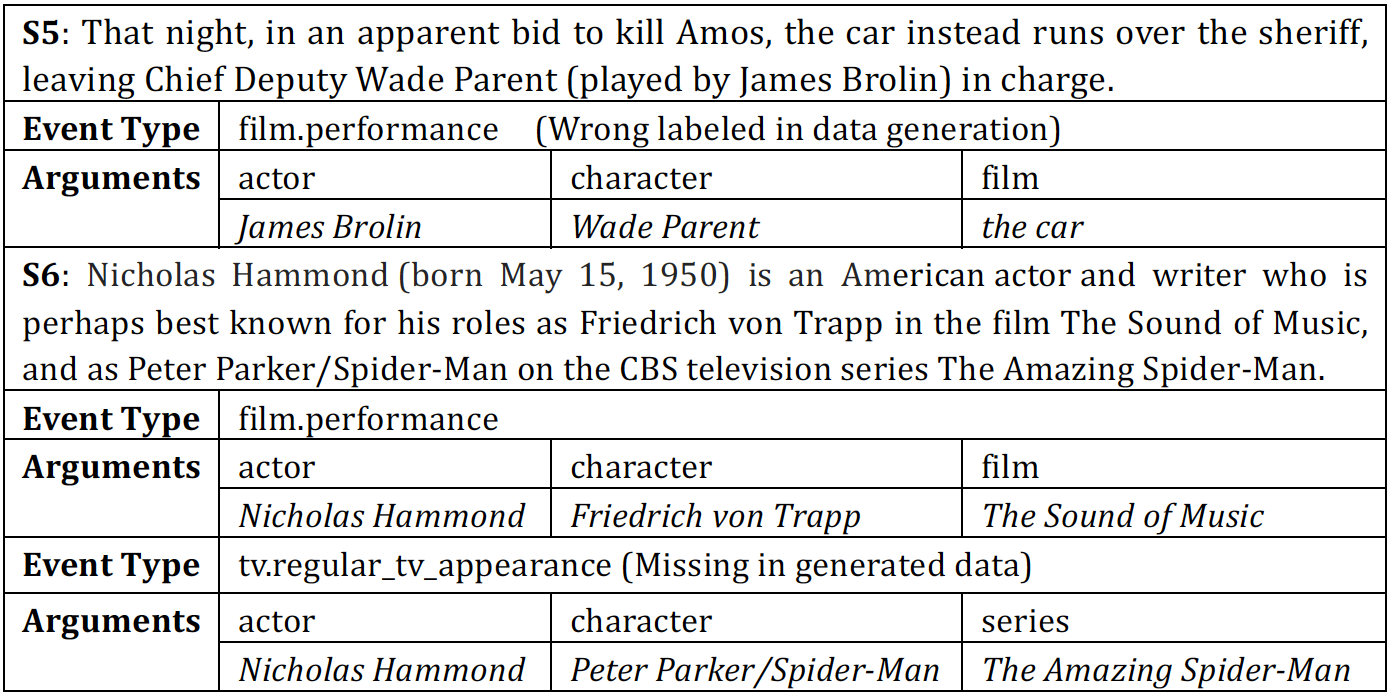
\includegraphics[width=.48\textwidth]{example.png}
	\caption{Example outputs of LSTM-CRF-ILP$_{multi}$.\label{fig:1}}
\end{figure}

We can draw similar conclusions about the comparison of performances between different models as automatic evaluation. We demonstrate that LSTM-CRF-ILP$_{multi}$ is the most effective model in event extraction as it attains the highest F1 score in both manual and automatic evaluation.

Moreover, manual evaluation helps us to gain a deep insight of our generated data and proposed models. We further conduct automatic evaluation on this manual annotated dataset and list the top 5 event types whose F1 scores of LSTM-CRF-ILP$_{multi}$ differ greatly from automatic evaluation in Table~\ref{tab:4}. 

\begin{table}[h]
\small
\centering
\begin{tabular}{|l|c|c|c|} \hline
	Event type & P & R & F \\ \hline
	olympics.medal\_honor \footnote{The full name is olympics.olympic\_medal\_honor in Freebase.} & $\downarrow$ 25.0\% & $\downarrow$ 5.0\% & $\downarrow$ 13.8\% \\ \hline
	film.performance & $\downarrow$ 21.4\% & $\uparrow$ 3.1\% & $\downarrow$10.3\% \\ \hline
	business.acquisition & $\rightarrow$ & $\downarrow$ 7.1\% & $\downarrow$ 5.4\% \\ \hline
	tv.appearance \footnote{The full name is tv.regular\_tv\_appearance in Freebase.} & $\downarrow$ 9.5\% & $\uparrow$ 3.0\% & $\downarrow$ 3.1\% \\ \hline
	film.release \footnote{The full name is film.film\_regional\_release\_date in Freebase.} & $\downarrow$ 7.7\% & $\uparrow$ 5.6\% & $\downarrow$ 0.55\% \\ \hline
\end{tabular}
\caption{Top 5 event types whose performances on event classification differ most from automatic evaluation. The model we evaluated is LSTM-CRF-ILP$_{multi}$ \label{tab:4}}
\end{table}

Most of the performance differences blame on the stage of data generation. Figure~\ref{fig:1} examples two types of errors in data generation. Some of the sentences automatic generated test set are noisy, in other words, they do not imply any event while still match all key properties of certain instances. Take S5 as an example, though the phrases \emph{the car} matches a film name, it does not indicate this film, and there is no explicit evidence expressing that an actor starring in a film. This is a bottleneck of our data generation strategy. During manual evaluation, we find 16 negative sentences and all of them are mistakenly labeled due to the same reason. Unfortunately, our model fails to identify some of these negative sentences.

Remarkably, our LSTM-CRF-ILP$_{multi}$ model can help find more CVT instances that not referenced in Freebase. There are two events mentioned in S6, while the arguments of the second event do not match any CVT instances in Freebase, leading to an omitting event in data generation. This phenomenon suggests that learning from distant supervision provided by Freebase, our model can help complete and update properties of Freebase instances in return.

\section{Related Work}
%Event extraction is one of the fundamental tasks in information extraction. % and natural language understanding. 
Most event extraction works are within the tasks defined by several evaluation frameworks (e.g., MUC~\cite{grishman1996message}, 
ACE~\cite{doddington2004automatic}, ERE~\cite{song2015light} and TAC-KBP~\cite{mitamura2015event}), 
all of which can be considered as a template-filling-based extraction task.
These frameworks focus on limited number of event types, which are designed and annotated by human experts and
hard to generalize to other domains.  
%Most approaches within  these frameworks 
Furthermore, existing extraction systems, which usually adopt a supervised learning paradigm, 
have to rely on those high-quality training data within those frameworks, 
thus hard to move to more domains in practice, regardless of feature-based~\cite{gupta2009predicting,hong2011using,li2013joint} or neural-network-based methods~\cite{chen2015event,nguyen2016joint}.

Besides the works focusing on small human-labeled corpus, 
Huang et al. \shortcite{huang2016liberal}  propose a novel Liberal Event Extraction paradigm 
which automatically discovers event schemas and extract events simultaneously from any unlabeled corpus. 
In contrast, we propose to exploit existing structured knowledge bases, e.g., Freebase, to automatically discover 
types of events as well as their corresponding argument settings, without expert annotation, and further automatically
construct training data, with the essence of distant supervision~\cite{mintz2009distant}.

Distant supervision~(\texttt{DS}) has been widely used in binary relation extraction, where the key assumption is that 
 sentences containing both the subject and object of a $<$$subj$, $rel$, $obj$$>$ triple can be seen as its support, and further
used to train a classifier to identify the relation $rel$. However,  this assumption does not fit to our event extraction scenario, 
where an event usually involves several arguments and it is hard to collect enough training sentences with all arguments appearing in, as indicated by the low coverage of \textbf{H1}. We therefore investigate different hypotheses  for event extraction within the \texttt{DS} paradigm and propose to utilize time and syntactic clues to refine the \texttt{DS} assumption for better data quality. We further relieve the reliance on event trigger annotations by previous event extractors, and define a novel event extraction paradigm with key arguments to characterize an event type. 

 
%
%However, these the reliance on high-quality training data are usually  human-annotated, and  training data prevents  
%
%We typically divide them into feature-based methods and neural-network-based methods. 
%
%Most traditional feature-based methods %usually rely on a variety of elaborate features. They 
% aim to exploit different feature extraction strategies and evaluate their contributions. 
%Besides training classifiers for each subtask, there are also works  jointly learning trigger labeling 
%and argument labeling using structured prediction models to capture both local and global 
%features of triggers and arguments~\cite{li2013joint}. 
%
%Neural-network-based methods are free of hard feature engineering and error propagation from  external NLP tools. 
%In the neural-network side, both convolutional neural network (CNN)~\cite{chen2015event}  and RNN have been employed 
%to extract features of different levels. 
%avoid hard feature engineering and error propagation from  external NLP tools. 
%Two types of neural works have been employed. Chen et al. \shortcite{chen2015event} 
%propose a convolutional neural network (CNN) with a dynamic multi-pooling layer to capture sentence-level features better. 
%Nguyen et al. \shortcite{nguyen2016joint} benefit from  a bidirectional RNN with various memory 
%matrices to jointly learn triggers and arguments within the ACE framework.% which benefits from both joint models and neural network  models. 
%However, to our knowledge, LSTM-CRF models have not been applied in earlier studies.
%
%In contrast to these prior systems focused on small human-labeled corpus, Huang et al. \shortcite{huang2016liberal} 
%propose a novel Liberal Event Extraction paradigm which automatically discovers event schemas and extract events 
%simultaneously from any unlabeled corpus. 


\section{Conclusions and Future Work}
Motivated by the data labeling problem in ACE event extraction system, we explore a method to generate training data automatically based on four hypotheses between arguments and events. The manual evaluation result demonstrates that our hypotheses are feasible, and the produced dataset is clean and high-quality.

In addition, we propose a LSTM-CRF model with a ILP-based post inference approach to perform event extraction on the auto-generated data. Experimental results of both manual and automatic evaluation show that our model can not only extract simple events, but also multi-type events and multiple events within one sentence.

Furthermore, we find that our model can extract information not collected by Freebase. In the future, we intend to explore an approach to extend this work to knowledge base population. 

% \section*{Acknowledgments}

%% The file named.bst is a bibliography style file for BibTeX 0.99c
\bibliographystyle{named}
\bibliography{ijcai17}

\end{document}

